\section{Architecture générale}
\label{archi:general}

\begin{figure}[H]
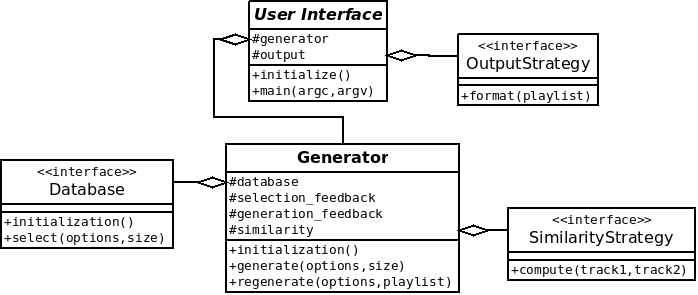
\includegraphics[width=\textwidth]{data/archi/general.png}
\caption{Diagramme général simplifié.}
\end{figure}

\section{Communication entre modules~: Morceaux et Options}
\label{archi:communication}

\subsection{Morceaux}
\label{archi:communication:track}

\begin{figure}[H]
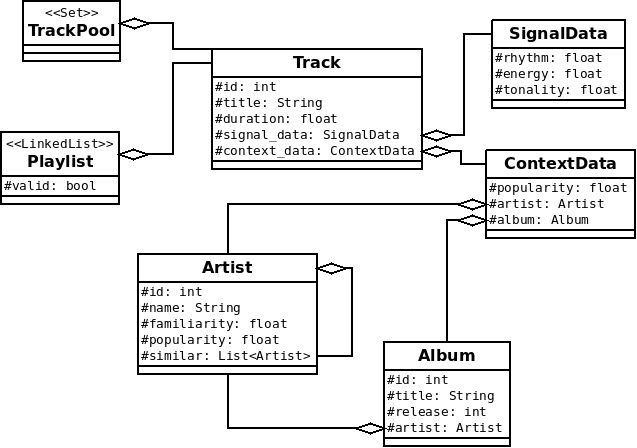
\includegraphics[width=\textwidth]{data/archi/track.png}
\caption{Diagramme des classes constituant un morceau.}
\end{figure}

\subsection{Options:~ La classe OptionList}
\label{archi:communication:options}

\section{Génération}
\label{archi:generation}

\begin{figure}[H]
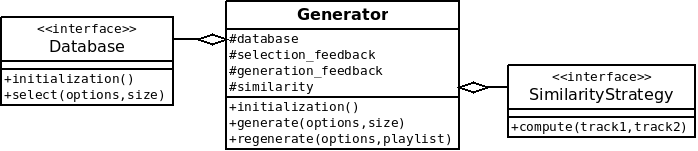
\includegraphics[width=\textwidth]{data/archi/generator.png}
\caption{Diagramme des classes du générateur.}
\end{figure}

\subsection{Le cœur de la génération~: La classe Generator}
\label{archi:generation:generator}

\subsection{Interface avec les données~: L'interface IDatabase}
\label{archi:generation:database}

\subsection{Stratégie de similarité~: l'interface ISimlarityStrategy}
\label{archi:generation:similarity}

\section{Module de sortie}
\label{archi:sortie}

\section{Interface Utilisateur}
\label{archi:interface}

\subsection{Retour utilisateur}
\label{archi:interface:feedback}

\begin{figure}[H]
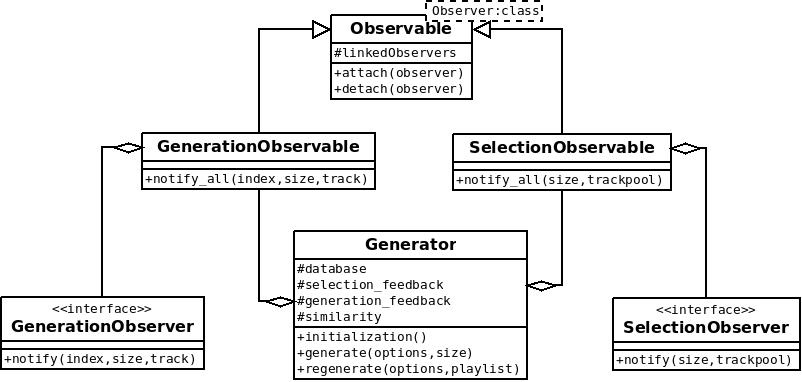
\includegraphics[width=\textwidth]{data/archi/feedback.png}
\caption{Diagramme des classes servant au retour utilisateur.}
\end{figure}

\begin{figure}[H]
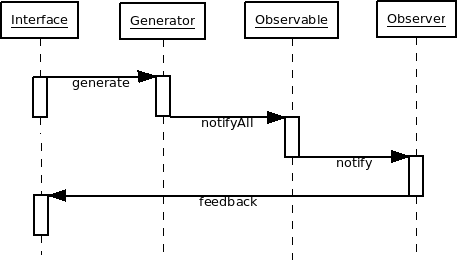
\includegraphics[width=\textwidth]{data/archi/feedback_sequence.png}
\caption{Diagramme de séquence du retour utilisateur.}
\end{figure}
>>>>>>> Stashed changes
